\chapter{Referencial Teórico}
\label{chap:refteo}

Neste capítulo, serão definidos os principais conceitos que fundamentam o presente trabalho, com destaque para \nameref{comele}, mais precisamente Comércio Eletrônico Móvel; \nameref{usabi} e \nameref{expusua}. Por fim, tem-se o \nameref{resteo}.

\section{Comércio Eletrônico} \label{comele}

O comércio eletrônico, conhecido como \textit{e-commerce}, abrange um vasto leque de atividades comerciais realizadas pela internet, envolvendo transações comerciais em que as partes interagem eletronicamente, em contraste com trocas físicas ou contato direto. Geralmente, é associado à compra e à venda via internet ou qualquer transação que envolva a transferência de propriedade ou direitos de uso de bens ou serviços por meio de uma rede mediada por computador. Contudo, essa definição, embora popular, não é abrangente o suficiente para abarcar os avanços recentes desse fenômeno comercial revolucionário. Uma definição mais abrangente considera o comércio eletrônico como a utilização de comunicações eletrônicas e tecnologias digitais de processamento de informações em transações comerciais, visando criar, transformar e redefinir relacionamentos para a geração de valor entre organizações, bem como entre organizações e indivíduos \citeonline{HongyanEcommerce}.

O rápido crescimento do comércio eletrônico tem sido constante desde sua origem. Uma de suas notáveis características de negócio é sua capacidade de permitir que pequenos comerciantes alcancem uma ampla base de consumidores, independentemente da proximidade geográfica, de acordo com \citeonline{MendoncaEcommerce}.

Nos últimos dois anos, houve uma transformação razoável no comportamento das pessoas, em particular motivada pela pandemia da COVID-19. Para os autores \citeonline{BaloghSustainable}, essa mudança comportamental é explicada como uma resposta a um evento estressante na vida dos consumidores, resultando na aceitação, intensificação ou alteração dos padrões de consumo como forma de lidar com o medo e a ansiedade. Essa influência reflete-se no notável aumento no comércio \textit{online}, evidenciando uma modificação nos hábitos de compra. Isso ocorre tanto em países desenvolvidos quanto em países em desenvolvimento. Nos EUA, por exemplo, houve um aumento de 32,4\% nas receitas \textit{online} em 2020. Já em locais como Bangladesh, onde as compras \textit{online} antes não dominavam o cenário, agora vivenciam um crescimento de 27\% nesse tipo de transação.

O comércio eletrônico pode funcionar de diversas maneiras tendo suas classificações nos seguintes tipos \cite{MendoncaEcommerce}:

\begin{itemize}
    \item \textbf{\textit{Business to Business (B2B)}}: Refere-se à relação comercial entre duas empresas, ocorrendo por meio de redes privadas compartilhadas entre elas;
    \item \textbf{\textit{Business to Consumer (B2C)}}: É o formato mais conhecido, envolvendo a venda direta de fabricantes ou distribuidores para o consumidor final;
    \item \textbf{\textit{Business to Employee (B2E)}}: Consiste na criação de plataformas pelas empresas para oferecer produtos aos funcionários a preços mais acessíveis;
    \item \textbf{\textit{Business to Government (B2G)}}: É quando uma empresa vende para o Governo;
    \item \textbf{\textit{Consumer to Business (C2B)}}: Consiste em um modelo onde os consumidores oferecem seus produtos ou serviços para as empresas, e
    \item \textbf{\textit{Consumer to Consumer (C2C)}}: Nesse formato, a transação ocorre entre consumidores, mediada por plataformas especializadas;
\end{itemize}

O comércio eletrônico oferece uma série de benefícios para os consumidores. De acordo com \citeonline{ECommerceOverview}, uma de suas principais vantagens, do ponto de vista do cliente, estabelece-se na grande melhoria e economia de tempo, permitindo acessibilidade e conveniência a partir de qualquer local do mundo. Alguns dos benefícios primordiais para os consumidores incluem: 

\begin{itemize}
    \item Maior flexibilidade, possibilitando compras 24 horas por dia sem necessidade de contato físico com a empresa;
    \item Economia de tempo, oferecendo a oportunidade de comprar ou vender produtos a qualquer momento \textit{online};
    \item Facilidade de acesso às informações, proporcionando aos consumidores a conveniência de pesquisar detalhes em várias páginas com um simples clique, permitindo acesso contínuo e conveniente aos dados;
    \item Conforto, pois as compras e transações podem ser realizadas no ambiente mais conveniente para o comprador, seja em casa ou no escritório;
    \item Facilidade de mudança para outras empresas-clientes, caso a operação da empresa atual seja insatisfatória;
    \item Acesso a produtos indisponíveis no mercado local ou nacional, ampliando o alcance de produtos disponíveis para os clientes, e
    \item Maior conhecimento sobre análises e avaliações o de produtos por meio de comentários de outros compradores, permitindo ao consumidor avaliar a experiência de outros clientes antes de realizar a compra final.
\end{itemize}

Um ponto adicional a ser destacado é que o termo comércio eletrônico surgiu quando o principal acesso aos produtos e serviços oferecidos de forma \textit{online} eram realizados por \textit{desktops} e \textit{laptops/notebooks}. Entretanto, nos tempos modernos, o comércio eletrônico tem sido acessado, principalmente, via dispositivos móveis, tais como celulares e \textit{tablets}. Nesse sentido, surge um novo conceito, o chamado comércio móvel \textit{(m-commerce)} \cite{LucasAlmeida}, o qual compartilha da mesma definição do comércio eletrônico. Entretanto, tem a particularidade de conferir ênfase aos diferentes modos de acesso, ou seja, via diferentes dispositivos móveis. Isso impõe novos desafios, uma vez que vários desses dispositivos possuem telas com tamanhos e resoluções diferentes, além de variadas capacidades de memória e processamento. Essas são algumas das demandas extras impostas às plataformas que oferecem produtos e serviços \textit{online}. No presente trabalho, o maior olhar será para o comércio móvel, doravante referenciado como comércio eletrônico móvel. A ideia é manter o elo com o comércio eletrônico, mas conferindo ao leitor um olhar mais focado nesse acesso amplo, via dispositivos móveis.

Conforme colocado anteriormente, demandas extras são impostas pelo comércio eletrônico móvel. Cabe, nesse contexto, reportar as mais relevantes, de acordo com \citeonline{ComputacaoMovel} e \citeonline{ComunicacaoEComputacao}:

\begin{itemize}
    \item \textbf{Interface com Dispositivos Móveis}: normalmente, esses dispositivos possuem telas reduzidas, ausência de teclados tradicionais, e até mesmo ausência de dispositivos auxiliares (ex. \textit{mouse}). Sendo assim, são dispositivos mais mais limitados, e que precisam ser considerados com suas particularidades;
    
    \item \textbf{Capacidade dos Dispositivos Móveis}: novamente, esses dispositivos possuem recursos restritos de processamento e memória. Conteúdos muito adensados para serem baixados, acessados, podem dificultar muito o uso desses dispositivos;
    
    \item \textbf{Segurança}: esses dispositivos acessam as plataformas \textit{online} via rede sem fio. Essas redes estão mais sujeitas a ataques maliciosos, com maior possibilidade dos dados serem interceptados facilmente, caso não ocorra um adequado cuidado em termos de autenticação/autorização e criptografia, e
    
    \item \textbf{Adaptabilidade}: esses dispositivos demandam soluções que levem em consideração as caraterísticas físicas e pessoas. Por características físicas, têm-se, por exemplo, a possível desconexão do cliente em meio a uma transação, enquanto movendo-se com o dispositivo. Por características pessoas, têm-se, por exemplo, a necessidade de lidar com informações de localização, que podem variar, devido à mobilidade conferida pelo dispositivo móvel.
\end{itemize} 


\subsection{Comércio Eletrônico no Brasil}

No Brasil, a empresa pioneira em conduzir seu negócio nos moldes de comércio eletrônico foi a Magazine Luíza. Isso ocorre em março de 1992, dois anos após o lançamento da \textit{World Wide Web} e antes da disponibilidade da internet no país, que só foi oficialmente liberada pelo Ministério das Comunicações em 1995. Esse modelo inicial foi aprimorado e mais tarde transformado em uma plataforma de loja virtual. No contexto virtual, a primeira loja virtual no Brasil foi estabelecida pela Brasoftware, desenvolvida em 1996 por Ricardo Jordão Magalhães. Até o ano de 2001, os dados estatísticos sobre o comércio eletrônico no Brasil eram inexistentes. Foi quando surgiu a empresa Ebit\footnote{\url{https://www.ebit.com.br/}}, que começou a monitorar e registrar o faturamento do comércio eletrônico brasileiro, fornecendo um panorama mais claro sobre a indústria \cite{MendoncaEcommerce}.

Um estudo muito importante conduzido pela \citeonline{RelatoriosEbit} é o relatório \textit{Webshoppers} que, desde 2001, destaca-se como a principal fonte de credibilidade no que diz respeito ao comércio eletrônico brasileiro, sendo amplamente considerado como referência primordial para os profissionais atuantes nesse segmento. Através de dados desse relatório, por exemplo, é possível compreender o crescimento do comércio eletrônico antes, durante e após a pandemia.

Analisando os gráficos apresentados a seguir, é possível compreender o quanto a pandemia impulsionou o crescimento do comércio eletrônico. O gráfico da Figura \ref{fig01} apresenta números que comprovam que o faturamento do primeiro semestre de 2020 foi 9\% maior que o segundo semestre de 2019. Já o gráfico da Figura \ref{fig02}, mostra um crescimento, comparando antes da pandemia, com 16\%, e durante o período de COVID-19, com 57\%. Nessa mesma ilustração, são reveladas as datas comemorativas, as quais representam forte expansão para vendas \textit{online}, tais como: o dia do consumidor e a páscoa. Isso justifica o aumento a partir de abril.

\begin{figure}[h]
    \centering
    \caption{Recorde de faturamento em 20 anos de comércio eletrônico no Brasil no 1/2020}
    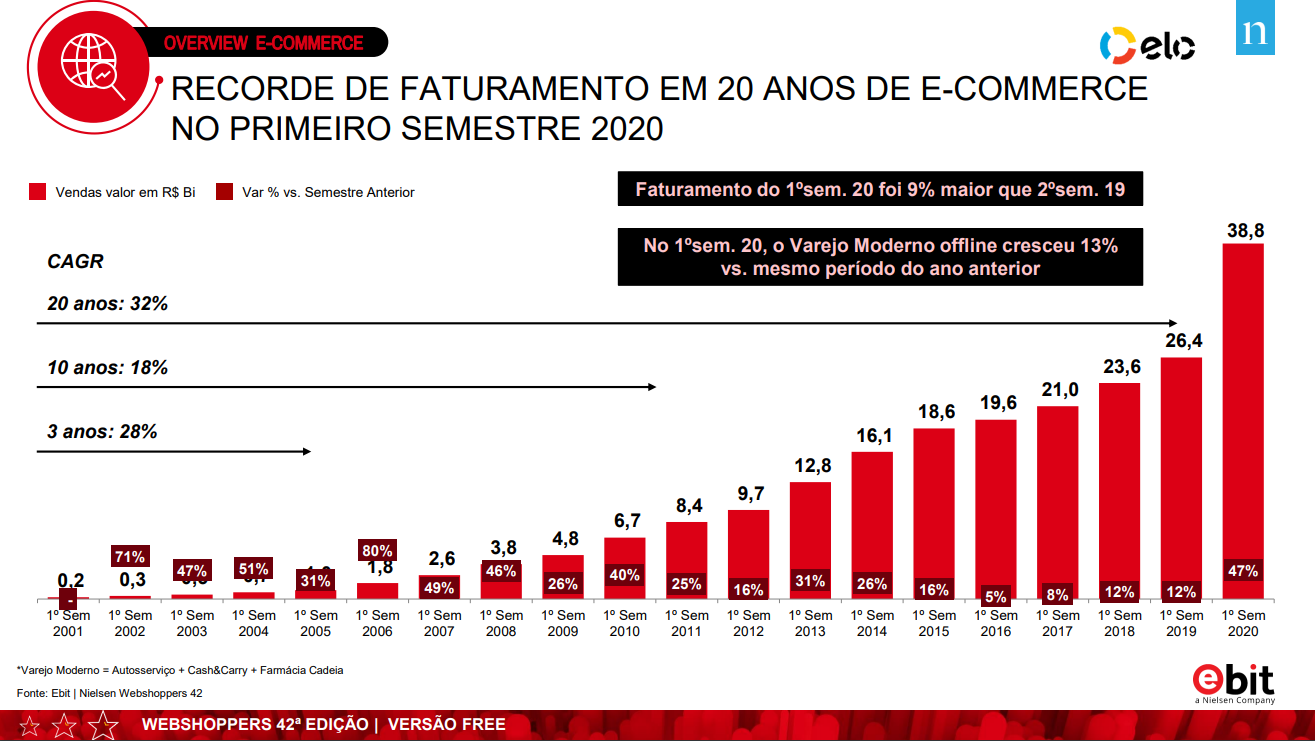
\includegraphics[keepaspectratio=true,scale=0.3]{figuras/edicao42.png}
    \legend{Fonte: \textit{Webshoppers} Edição 42, Ebit | Nielsen}
    \label{fig01}
\end{figure}

\begin{figure}[h]
    \centering
    \caption{Crescimento intenso do comércio eletrônico durante a pandemia no Brasil}
    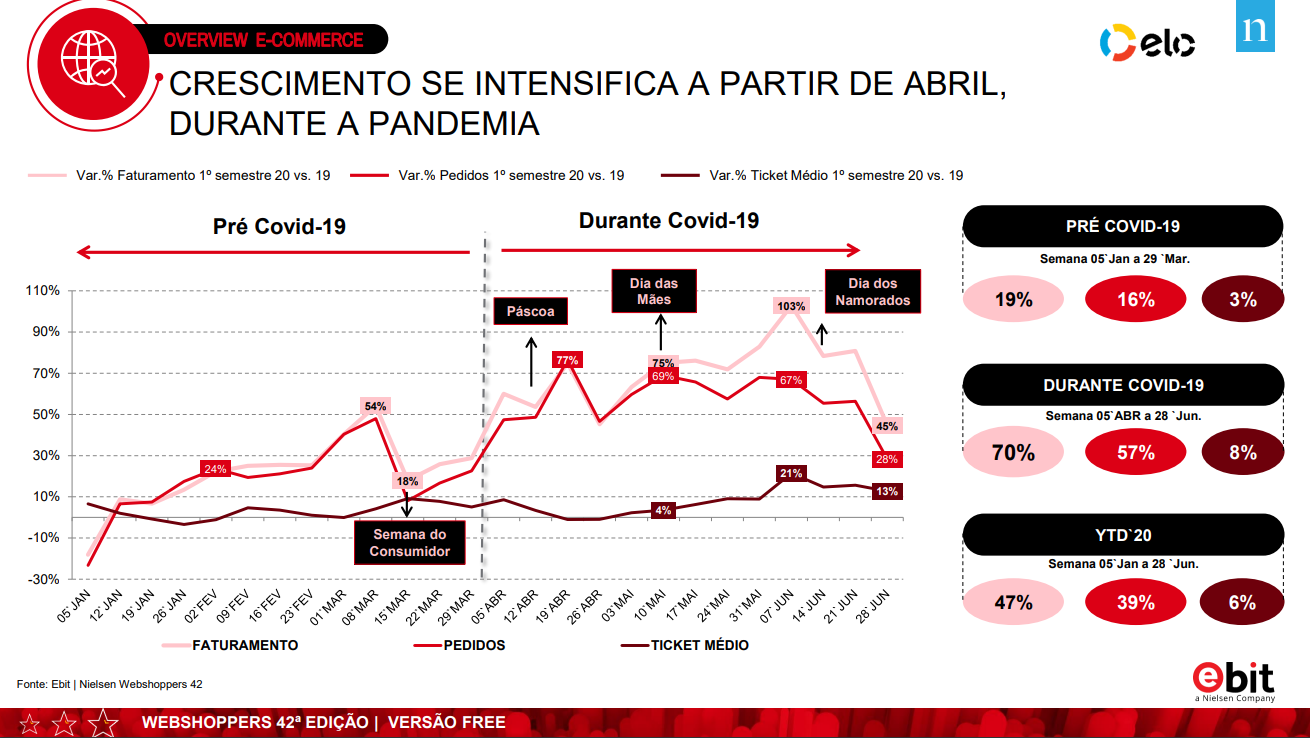
\includegraphics[keepaspectratio=true,scale=0.3]{figuras/edicao42a.png}
    \legend{Fonte: \textit{Webshoppers} Edição 42, Ebit | Nielsen}
    \label{fig02}
\end{figure}

O gráfico da Figura \ref{fig03} é de uma pesquisa realizada em agosto de 2023, onde mostra que o comércio eletrônico possui atualmente 53 milhões de consumidores. Com esses dados, fica evidente não apenas o crescimento do negócio, mas também como é vantajoso para a empresa investir na experiência de usuário dentro de sua plataforma.

\begin{figure}[h]
    \centering
    \caption{Evolução de consumidores no comércio eletrônico}
    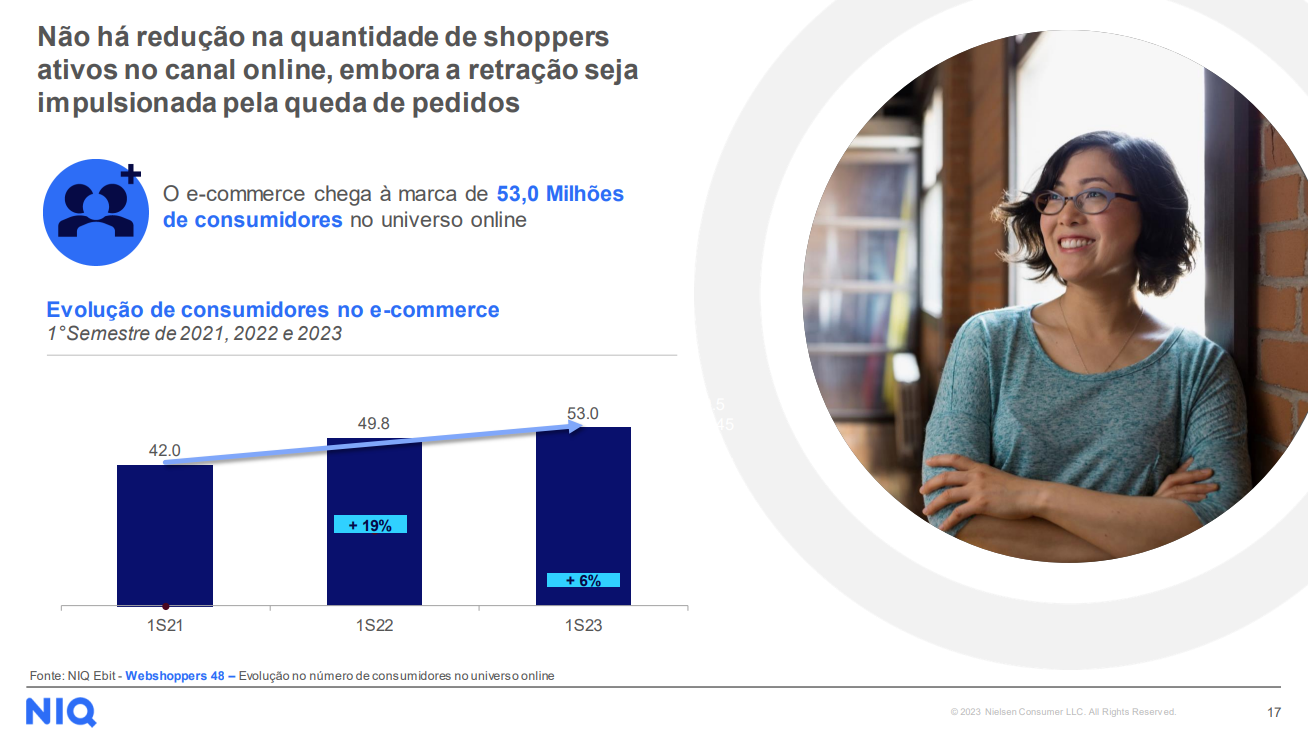
\includegraphics[keepaspectratio=true,scale=0.3]{figuras/edicao48.png}
    \legend{Fonte: \textit{Webshoppers} Edição 48, Ebit | Nielsen}
    \label{fig03}
\end{figure}



\section{Usabilidade} \label{usabi}

Em \citeonline{ISO924210}, há uma definição sobre usabilidade, sendo essa a medida em que um sistema, produto ou serviço pode ser utilizado por usuários para atingir objetivos específicos com eficácia, eficiência e satisfação, dentro de um contexto de uso particular. Além disso, o termo ``usabilidade'' é empregado como qualificador para descrever o conhecimento de \textit{design}, habilidades e atividades envolvidas. Isso inclui áreas como experiência em usabilidade, profissionais de usabilidade, engenharia de usabilidade, métodos de usabilidade, avaliação de usabilidade e heurísticas de usabilidade.

Segundo \citeonline{NNGroupUI}, a usabilidade é definida por cinco componentes de qualidade:

\begin{itemize}
    \item \textbf{Aprendizagem}: Qual é a facilidade para os usuários realizarem tarefas básicas na primeira vez em que se deparam com o \textit{design}?
    \item \textbf{Eficiência}: Depois que os usuários aprendem o \textit{design}, com que rapidez eles conseguem realizar as tarefas?
    \item \textbf{Memorização}: Quando os usuários retornam ao \textit{design} após um período sem usá-lo, com que facilidade eles conseguem restabelecer a proficiência?
    \item \textbf{Erros}: Quantos erros os usuários cometem, bem como qual é a gravidade desses erros e com que facilidade eles conseguem se recuperar dos erros?
    \item \textbf{Satisfação}: Qual é o grau de prazer em usar o \textit{design}?
\end{itemize}

Assim como são utilizados guias para garantir uma boa usabilidade ao usuário, é necessários também utilizar métodos para examinar se estão sendo seguidos. Também segundo \citeonline{NNGroupUI}, o teste de usuário é um dos mais fundamentais e e práticos métodos utilizados para saber se a usabilidade é adequada, mas sempre tendo o cuidado de selecionar usuários representativos como clientes para um site de comércio eletrônico. Adicionalmente, deve-se pedir aos usuários que executem tarefas que reflitam o uso real do \textit{design}, observando as ações dos usuários, afim de identificar áreas de sucesso e de dificuldade na interação com a interface. Por fim, cabe ressaltar ser muito relevante permitir que os usuários atuem de maneira independente, sem intervenções que possam influenciar os resultados do teste.

Uma visão geral sobre testes de usabilidade pode ser encontrada em \citeonline{KatiaTesteTCC} e \citeonline{LewisHandbook}. Dentre os aspectos mencionados pelos autores, destacam-se: exemplos de testes de usabilidade, ilustrados via cenários de uso, e preocupações quanto à efetividade desses testes. Mas, ainda assim, os autores recomendam seu uso. Como a intenção deste trabalho centra-se na experiência de usuário, o olhar da usabilidade será voltado para aspectos que impactam experiência de usuário. Nesse sentido, serão consideradas as Heurísticas de Nielsen \cite{HeuristicasNielsen}.

\subsection{Heurísticas de Nielsen}
\label{HeuristicasNielsen}

As heurísticas de Nielsen representam um método para examinar o \textit{design} da interface, destacando possíveis falhas e equívocos a fim de corrigi-los e aprimorando a experiência do usuário (UX). Sendo assim, os princípios gerais de \citeonline{HeuristicasNielsen} para o \textit{design} de interação consistem em diretrizes abrangentes que fornecem orientações essenciais para a usabilidade. Em linhas gerais, as heurísticas consistem em:

\begin{enumerate}
    \item \textbf{Visibilidade do status do sistema}: Manter os usuários informados sobre as ações em curso, oferecendo \textit{feedback} adequado em um intervalo de tempo razoável. Por exemplo, ;
    \item \textbf{Correspondência entre o sistema e o mundo real}: Utilizar linguagem familiar aos usuários, evitando jargões internos. O \textit{design} deve seguir convenções do mundo real para facilitar a compreensão dos usuários. Por exemplo, ;
    \item \textbf{Controle e liberdade do usuário}: Oferecer uma "saída de emergência" claramente indicada permite que os usuários desfaçam ações indesejadas. Por exemplo, ;
    \item \textbf{Consistência e padrões}: Evitar ambiguidades, garantindo que diferentes palavras ou ações signifiquem a mesma coisa. Seguir convenções da plataforma e do setor é essencial, como a localização consistente dos balcões de \textit{check-in} em hotéis;
    \item \textbf{Prevenção de erros}: Além de fornecer boas mensagens de erro, um \textit{design} adequado evita problemas desde o início, eliminando situações propensas a erros. Por exemplo, ;
    \item \textbf{Reconhecimento em vez de recordação}: Minimizar a carga de memória do usuário ao tornar elementos, ações e opções visíveis. Informações necessárias devem ser facilmente acessíveis. Por exemplo, ;
    \item \textbf{Flexibilidade e eficiência de uso}: Oferecer atalhos que aceleram a interação para usuários experientes sem sobrecarregar iniciantes. Permitir personalização de ações frequentes. Por exemplo, ;
    \item \textbf{\textit{Design} estético e minimalista}: Evitar informações irrelevantes ou excessivas que possam distrair ou competir com dados essenciais. Por exemplo, ;
    \item \textbf{Ajuda os usuários a reconhecer, diagnosticar e se recuperar de erros}: Mensagens de erro claras e construtivas ajudam os usuários a identificar e resolver problemas. Por exemplo, e
    \item \textbf{Ajuda e documentação}: O ideal é que o sistema seja autoexplicativo, mas se necessário, fornecer documentação para ajudar os usuários a entender como concluir tarefas. Por exemplo, .
\end{enumerate}

\section{Experiência de Usuário} \label{expusua}

De acordo com a \citeonline{ISO924210}, a experiência do usuário ou \textit{User Experience} (UX) surge da apresentação, funcionalidade e desempenho do sistema, assim como do comportamento interativo e dos recursos de apoio presentes em um sistema interativo. Sendo assim, têm-se percepções e respostas do usuário que resultam do uso e/ou do uso previsto de um sistema, produto ou serviço, incluindo suas emoções, crenças, preferências, conforto, comportamentos e realizações que ocorrem antes, durante e depois do uso. A experiência do usuário é uma consequência da imagem da marca, da apresentação, da funcionalidade, do desempenho do sistema, do comportamento interativo e dos recursos de assistência de um sistema, produto ou serviço. Ela também é resultado dos estados interno e físico do usuário, resultante de experiências anteriores, atitudes, habilidades, capacidades e personalidade, além do contexto de uso.

\subsection{Avaliação da Experiência de Usuário usando AttrakDiff} \label{adiff}

Durante as avaliações de UX, os usuários testam a aplicação e expressam suas experiências ao utilizá-la. Segundo \citeonline{EstudoPráticoAttrakDiff}, essa forma de avaliação permite que empresas de software desenvolvam aplicativos comercialmente viáveis, focando nas necessidades e emoções dos usuários. Tendo como objetivo é compreender as emoções dos usuários ao usar a aplicação, medir suas satisfações e avaliar as experiências de uso são ações relevantes. Diversos métodos de UX são propostos para atingir tais metas. Dentre os métodos comumente adotados para avaliação de UX, está o questionário \textit{AttrakDiff}, fundamentado no modelo de experiência do usuário de \citeonline{AttrakDiff}. No contexto do presente trabalho, esse questionário foi escolhido para avaliar a experiência dos usuários, pois permite uma análise da qualitativa de uma aplicação por meio de diferentes aspectos.

O \textit{AttrakDiff} é um questionário constituído por 28 pares de palavras, sendo dividido em três dimensões: a Qualidade Pragmática (QP); a Qualidade Hedônica, que possui as subdivisões Estímulo (QH–E) e Identidade (QE–I), e por fim, a  Atratividade (AT).

\begin{itemize}
    \item \textbf{Qualidade Pragmática (QP)}: Essa dimensão avalia o desempenho geral de uma aplicação, e reflete o quão bem os usuários conseguem alcançar seus objetivos ao usar essa aplicação;
    \item \textbf{Qualidade Hedônica-Estímulo (QH-E)}: Essa dimensão observa em que medida a aplicação é capaz de satisfazer as necessidades de evolução e crescimento, oferecendo elementos de originalidade, interesse e estímulo;
    \item \textbf{Qualidade Hedônica-Identidade (QH-I)}: Essa dimensão analisa o quão bem a aplicação permite que os usuários se identifiquem e se conectem com ela, e
    \item \textbf{Atratividade (AT)}: Esta dimensão avalia a percepção global de valor da aplicação, considerando a visão geral de qualidade percebida pelos usuários.
\end{itemize}

De acordo com \citeonline{AttrakDiffR}, o \textit{AttrakDiff} pode ser aplicado com sua versão mínima, que consiste em apenas 10 pares de palavras, ou o \textit{AttrakDiff-R}, que consiste em uma versão, também compacta, mas contendo 18 pares de palavras. Tendo isso em vista, será utilizado o \textit{AttrakDiff-R} para condução deste trabalho, contendo 18 pares de palavras numa escala de 7 pontos Likert, como ser observado no Quadro \ref{qAttrakDiff}.

A análise dos resultados pode ser realizada de três maneiras distintas segundo \citeonline{AttrakDiffR}:

\begin{itemize}
    \item Com a descrição dos pares de palavras, que apresenta os valores médios de cada par agrupados nas quatro dimensões;
    \item Com o portfólio dos resultados, que é composto por quadrantes que analisam o QPR e o QH, e
    \item Por um diagrama de valores médios, que apresenta a média das quatro dimensões do produto sob as quatro dimensões.
\end{itemize}

% \setfloatlocations{quadro}{hbtp}
\begin{quadro}
\caption{\label{qAttrakDiff}Pares de palavras do AttrakDiff}

\begin{tabular}{|c|cc|}
\hline
\textbf{Dimensão}             & \multicolumn{2}{c|}{\textbf{Par de Palavras}}                        \\ \hline
\multirow{5}{*}{\textbf{QPR}} & \multicolumn{1}{c|}{Técnico}                 & Humano                \\ \cline{2-3} 
                              & \multicolumn{1}{c|}{Complicado}              & Simples               \\ \cline{2-3} 
                              & \multicolumn{1}{c|}{Imprevisível}            & Previsível            \\ \cline{2-3} 
                              & \multicolumn{1}{c|}{Confuso}                 & Bem Estruturado       \\ \cline{2-3} 
                              & \multicolumn{1}{c|}{Incontrolável}           & Gerenciável           \\ \hline
\multirow{4}{*}{\textbf{QHE}} & \multicolumn{1}{c|}{Sem imaginação}          & Criativo              \\ \cline{2-3} 
                              & \multicolumn{1}{c|}{Cauteloso}               & Ousado                \\ \cline{2-3} 
                              & \multicolumn{1}{c|}{Entediante}              & Chamativo             \\ \cline{2-3} 
                              & \multicolumn{1}{c|}{Pouco Exigente}          & Desafiador            \\ \hline
\multirow{5}{*}{\textbf{QHI}} & \multicolumn{1}{c|}{Não profissional}        & Profissional          \\ \cline{2-3} 
                              & \multicolumn{1}{c|}{Não apresentável}        & Apresentável          \\ \cline{2-3} 
                              & \multicolumn{1}{c|}{De baixa qualidade}      & De alta qualidade     \\ \cline{2-3} 
                              & \multicolumn{1}{c|}{Alienador}               & Integrador            \\ \cline{2-3} 
                              & \multicolumn{1}{c|}{Me aproxima das pessoas} & Me afasta das pessoas \\ \hline
\multirow{4}{*}{\textbf{ATT}} & \multicolumn{1}{c|}{Decepcionado}            & Realizado             \\ \cline{2-3} 
                              & \multicolumn{1}{c|}{Feio}                    & Bonito                \\ \cline{2-3} 
                              & \multicolumn{1}{c|}{Mau}                     & Bom                   \\ \cline{2-3} 
                              & \multicolumn{1}{c|}{Desencorajador}          & Motivador             \\ \hline
\end{tabular}
\legend{Fonte: \cite{AttrakDiff}}
\end{quadro} 

Para coleta e análise dos dados, serão utilizados \textit{Google Forms} e \textit{Google Sheets}, tendo em vista que a plataforma original do \textit{AttrakDiff}, mesmo sendo disponibilizada de forma gratuita, funciona somente nos idiomas Alemão e Inglês. Como o público-alvo deste trabalho são pessoas brasileiras que falam português, torna-se inadequada a opção de utilizar o modelo original. Outros detalhes sobre o referencial tecnológico desse trabalho constam no próximo capítulo.

\section{Resumo do Capítulo} 
\label{resteo}

Este capítulo expôs os principais conceitos e fundamentos relacionados ao contexto do trabalho, sendo eles: Comércio Eletrônico, Usabilidade e Experiência de Usuário.
Na contextualização de Comércio Eletrônico, foi abordado a evolução do setor desde sua criação relatando suas diferentes classificações, assim como seu pico de crescimento durante a pandemia da COVID-19 expondo os benefícios do setor para os consumidores e apresentando o conceito de Comércio Eletrônico Móvel, que é o foco desde trabalho, sendo o comércio com foco em dispositivos móveis principalmente \textit{smartphones}. Finalizando o tópico com o cenário atual do Comércio Eletrônico atual no Brasil através de pesquisas e gráficos.

Em seguida, foi apresentada Usabilidade demostrando sua importância e expondo cinco componentes além de oito Heurísticas de qualidade. Por fim, foi abordado o conceito de Experiência do Usuário como fator essencial para o sucesso de um Comércio Eletrônico e também exposto o método de Avaliação usando \textit{AttrakDiff}.




